\XtoCBlock{TypeConv}
\label{block:TypeConv}
\begin{figure}[H]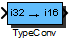
\includegraphics{TypeConv}\end{figure} 

\begin{XtoCtabular}{Inports}
In & \tabularnewline
\hline
\end{XtoCtabular}


\begin{XtoCtabular}{Outports}
Out & \tabularnewline
\hline
\end{XtoCtabular}

\subsubsection*{Description:}
Data Type Conversion

\subsubsection*{Implementations:}
\begin{tabular}{l l}
\textbf{FiP8\_16} & 8 to 16 Bit Fixed Point Implementation\tabularnewline
\textbf{FiP8\_32} & 8 to 32 Bit Fixed Point Implementation\tabularnewline
\textbf{FiP16\_8} & 16 to 8 Bit Fixed Point Implementation\tabularnewline
\textbf{FiP16\_32} & 16 to 32 Bit Fixed Point Implementation\tabularnewline
\textbf{FiP32\_8} & 32 to 8 Bit Fixed Point Implementation\tabularnewline
\textbf{FiP32\_16} & 32 to 16 Bit Fixed Point Implementation\tabularnewline
\end{tabular}

\XtoCImplementation{FiP8\_16}
\index{Block ID!176}
\nopagebreak[0]
% Implementation details
\begin{tabular}{l l}
\textbf{Name} & FiP8\_16 \tabularnewline
\textbf{ID} & 176 \tabularnewline
\textbf{Revision} & 0.1 \tabularnewline
\textbf{C filename} & TypeConv\_FiP8\_16.c \tabularnewline
\textbf{H filename} & TypeConv\_FiP8\_16.h \tabularnewline
\end{tabular}
\vspace{1ex}

8 to 16 Bit Fixed Point Implementation

% Implementation data structure
\XtoCDataStruct{Data Structure:}
\begin{lstlisting}
typedef struct {
     uint16        ID;
     int8          *In;
     int16         Out;
} TYPECONV_FIP8_16;
\end{lstlisting}

\ifdefined \AddTestReports
\InputIfFileExists{\XcHomePath/Library/General/Doc/Test_TypeConv_FiP8_16.tex}{}{}
\fi
\XtoCImplementation{FiP8\_32}
\index{Block ID!177}
\nopagebreak[0]
% Implementation details
\begin{tabular}{l l}
\textbf{Name} & FiP8\_32 \tabularnewline
\textbf{ID} & 177 \tabularnewline
\textbf{Revision} & 0.1 \tabularnewline
\textbf{C filename} & TypeConv\_FiP8\_32.c \tabularnewline
\textbf{H filename} & TypeConv\_FiP8\_32.h \tabularnewline
\end{tabular}
\vspace{1ex}

8 to 32 Bit Fixed Point Implementation

% Implementation data structure
\XtoCDataStruct{Data Structure:}
\begin{lstlisting}
typedef struct {
     uint16        ID;
     int8          *In;
     int32         Out;
} TYPECONV_FIP8_32;
\end{lstlisting}

\ifdefined \AddTestReports
\InputIfFileExists{\XcHomePath/Library/General/Doc/Test_TypeConv_FiP8_32.tex}{}{}
\fi
\XtoCImplementation{FiP16\_8}
\index{Block ID!178}
\nopagebreak[0]
% Implementation details
\begin{tabular}{l l}
\textbf{Name} & FiP16\_8 \tabularnewline
\textbf{ID} & 178 \tabularnewline
\textbf{Revision} & 0.1 \tabularnewline
\textbf{C filename} & TypeConv\_FiP16\_8.c \tabularnewline
\textbf{H filename} & TypeConv\_FiP16\_8.h \tabularnewline
\end{tabular}
\vspace{1ex}

16 to 8 Bit Fixed Point Implementation

% Implementation data structure
\XtoCDataStruct{Data Structure:}
\begin{lstlisting}
typedef struct {
     uint16        ID;
     int16         *In;
     int8          Out;
} TYPECONV_FIP16_8;
\end{lstlisting}

\ifdefined \AddTestReports
\InputIfFileExists{\XcHomePath/Library/General/Doc/Test_TypeConv_FiP16_8.tex}{}{}
\fi
\XtoCImplementation{FiP16\_32}
\index{Block ID!179}
\nopagebreak[0]
% Implementation details
\begin{tabular}{l l}
\textbf{Name} & FiP16\_32 \tabularnewline
\textbf{ID} & 179 \tabularnewline
\textbf{Revision} & 0.1 \tabularnewline
\textbf{C filename} & TypeConv\_FiP16\_32.c \tabularnewline
\textbf{H filename} & TypeConv\_FiP16\_32.h \tabularnewline
\end{tabular}
\vspace{1ex}

16 to 32 Bit Fixed Point Implementation

% Implementation data structure
\XtoCDataStruct{Data Structure:}
\begin{lstlisting}
typedef struct {
     uint16        ID;
     int16         *In;
     int32         Out;
} TYPECONV_FIP16_32;
\end{lstlisting}

\ifdefined \AddTestReports
\InputIfFileExists{\XcHomePath/Library/General/Doc/Test_TypeConv_FiP16_32.tex}{}{}
\fi
\XtoCImplementation{FiP32\_8}
\index{Block ID!180}
\nopagebreak[0]
% Implementation details
\begin{tabular}{l l}
\textbf{Name} & FiP32\_8 \tabularnewline
\textbf{ID} & 180 \tabularnewline
\textbf{Revision} & 0.1 \tabularnewline
\textbf{C filename} & TypeConv\_FiP32\_8.c \tabularnewline
\textbf{H filename} & TypeConv\_FiP32\_8.h \tabularnewline
\end{tabular}
\vspace{1ex}

32 to 8 Bit Fixed Point Implementation

% Implementation data structure
\XtoCDataStruct{Data Structure:}
\begin{lstlisting}
typedef struct {
     uint16        ID;
     int32         *In;
     int8          Out;
} TYPECONV_FIP32_8;
\end{lstlisting}

\ifdefined \AddTestReports
\InputIfFileExists{\XcHomePath/Library/General/Doc/Test_TypeConv_FiP32_8.tex}{}{}
\fi
\XtoCImplementation{FiP32\_16}
\index{Block ID!181}
\nopagebreak[0]
% Implementation details
\begin{tabular}{l l}
\textbf{Name} & FiP32\_16 \tabularnewline
\textbf{ID} & 181 \tabularnewline
\textbf{Revision} & 0.1 \tabularnewline
\textbf{C filename} & TypeConv\_FiP32\_16.c \tabularnewline
\textbf{H filename} & TypeConv\_FiP32\_16.h \tabularnewline
\end{tabular}
\vspace{1ex}

32 to 16 Bit Fixed Point Implementation

% Implementation data structure
\XtoCDataStruct{Data Structure:}
\begin{lstlisting}
typedef struct {
     uint16        ID;
     int32         *In;
     int16         Out;
} TYPECONV_FIP32_16;
\end{lstlisting}

\ifdefined \AddTestReports
\InputIfFileExists{\XcHomePath/Library/General/Doc/Test_TypeConv_FiP32_16.tex}{}{}
\fi
